  \documentclass[xcolor=table]{beamer}
\usepackage{beamerthemesplit}
\usepackage{wrapfig}
\usetheme{SPbGU}
\usepackage{pdfpages}
\usepackage{amsmath}
\usepackage{cmap} 
\usepackage[T2A]{fontenc} 
\usepackage[utf8]{inputenc}
\usepackage[english]{babel}
\usepackage{indentfirst}
\usepackage{amsmath}
\usepackage{tikz}
\usepackage{multirow}
\usepackage[noend]{algpseudocode}
\usepackage{algorithm}
\usepackage{algorithmicx}
\usepackage{fancyvrb}
\usetikzlibrary{shapes,arrows}
%usepackage{fancyvrb}
%\usepackage{minted}
%\usepackage{verbments}


\beamertemplatenavigationsymbolsempty

\title[Результаты группы за 2018 год]{Результаты группы за 2018 год}
\institute[СПбГУ]{
JetBrains Research, Programming Languages and Tools Lab  \\
Санкт-Петербургский Государственный Университет
}

\author[Семён Григорьев]{Семён Григорьев}

\date{15.12.2018}

\definecolor{orange}{RGB}{179,36,31}

\begin{document}
{
\begin{frame}[fragile]
  \begin{tabular}{p{2.0cm} p{7.5cm} p{1cm}}
   \begin{center}
      
\includegraphics[height=1.5cm]{pictures/jetbrainsResearch.pdf}
    \end{center}
    &
    \begin{center}
      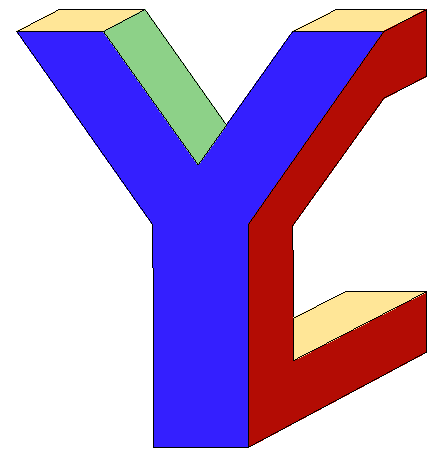
\includegraphics[height=1.5cm]{pictures/YC_logo.pdf}
    \end{center}
    &
    \begin{center}
      
\includegraphics[height=1.5cm]{pictures/SPbGU_Logo.png}
    \end{center} 
  \end{tabular}
  \titlepage
\end{frame}
}


\begin{frame}[fragile]
  \transwipe[direction=90]
  \frametitle{Группа}
\begin{itemize}
      \item Теория формальных языков
      \item Алгоритмы синтаксического анализа
      \item Применение теории флрмальных языков и синтаксического нализа для
      \begin{itemize}
        \item Статического анализа кода
        \item Анализа графовых баз даных
        \item Решения задач биоинформатики
      \end{itemize}

\end{itemize}

Состав: 1 аспирант, 3 магистра, 3 студента (``АУ'', ЛЭТИ, СПбГУ)
\end{frame}

\begin{frame}[fragile]
  \transwipe[direction=90]
  \frametitle{Научные конференции}
\begin{itemize}

      \item \textbf{ICFP-2018}
      \begin{itemize}
        \item Parser Combinators for Context-Free Path Querying (Scala simposium)
        \item F\# OpenCL C Type Provider (TyDe)
      \end{itemize}

      \item \textbf{SIGMOD-2018}
      \begin{itemize}
        \item Context-Free Path Querying by Matrix Multiplication (GRADES-NDA, доклад + пстер)
      \end{itemize}

      \item \textbf{BIATA-2018}
      \begin{itemize}
         \item 16s rRNA Detection by Using Neural Networks (постер)
      \end{itemize}
      
      \item \textbf{Современные технологии в теории и практике программирования}
      \begin{itemize}
         \item Контекстно чувствительный анализ алиасов
      \end{itemize}

\end{itemize}
\end{frame}
 
\begin{frame}[fragile]
  \transwipe[direction=90]
  \frametitle{Доклады}
\begin{itemize}

      \item \textbf{JetBrains Internal Conference-2018}
      \begin{itemize}
        \item Formal Languages Theory Is Not Only About Parsing
      \end{itemize}

      \item Доклад на семинаре по алгоритмической математике (ЛЭТИ, \url{http://pozdnkov.vm2-leti.spb.ru/iniciativy/proekty/seminar-po-algoritmiceskoj-matematike})

      \item Доклады на встерчах тематических групп (FProg, IT Global Meetup)

\end{itemize}
\end{frame}


\begin{frame}[fragile]
  \transwipe[direction=90]
  \frametitle{Публикации}
\begin{itemize}
      \item Материалы конференций
        \begin{itemize}
          \item \textbf{ICFP, SIGMOD} --- ACM
          \item Остальное --- сборники материалов конференций
        \end{itemize}
      \item Азимов Р. Ш., Григорьев С. В. Синтаксический анализ графов с использованием конъюнктивных грамматик // Труды института системного программирования РАН. – 2018. (ВАК)
\end{itemize}
\end{frame}

\begin{frame}[fragile]
  \transwipe[direction=90]
  \frametitle{Сотрудничество}
\begin{itemize}
      \item Грант РНФ под руководством Александра Охотина
      \item INRIA LINKS (\url{https://team.inria.fr/links/team-members/})
      \begin{itemize}
         \item Стажировка Рустама Азимова (сентябрь-ноябрь 2018)
         \item Планируется поездка в апреле 2019
      \end{itemize}
      \item Чтение курсов по теории формальных языков и теории графов на Математико-Механическом факультете СПбГУ
      \item Семинар по теории формальных языков
      \item Попытка применить теорию формальных языков для межпроцедурного анализа в рамках проекта ReSharper
      
\end{itemize}
\end{frame}

\begin{frame}[fragile]
  \transwipe[direction=90]
  \frametitle{Планируемые публикации}
\begin{itemize}
      \item Semyon Grigorev, Polina Lunina. The Composition of Dense Neural Networks and Formal Grammars for Secondary Structure Analysis. Подана на BIOINFORMATICS-2019
      \item Rustam Azimov, Semyn Grigorev. Path Querying with Conjunctive Grammars by Matrix Multiplication. Подана на LATA-2019
      \item Sergey Bozhko, Leyla Khatbullina, Semyon Grigorev. Bar-Hillel Theorem Mechanization in Coq. Подготовлена
\end{itemize}
\end{frame}


\end{document}
